\documentclass[superscriptaddress, twocolumn, prl, longbibliography, nofootinbib]{revtex4-1}
\usepackage{amsmath}
\usepackage{amsbsy}
\usepackage{amssymb}
\usepackage{graphicx}
\usepackage{color}
\usepackage{subfigure}
\usepackage{physics}
\usepackage{soul}
\usepackage{color}
\usepackage{bm}
\usepackage{array}
\usepackage{multirow}
\usepackage{lipsum}
\usepackage[normalem]{ulem}
%\newcommand{\Tr}{\text{Tr}}
\newcommand{\Ai}{\text{Ai}}
\newcommand{\Bi}{\text{Bi}}
\newcommand{\Real}{\text{Re}}
\newcommand{\Imag}{\text{Im}}
\usepackage{verbatim}
\usepackage{natbib}
\usepackage{nccmath}
\definecolor{linkcolor}{rgb}{0,0,0.6} 
\usepackage[pdftex,colorlinks=true,
	pdfstartview = FitV,
	linkcolor    = linkcolor,
	citecolor    = linkcolor,
	urlcolor     = linkcolor,	
	hyperindex   = true,
	hyperfigures = false]{hyperref}


\newcommand{\ee}{\text{e}}
\newcommand{\A}{\text{\tiny{A}}}
\newcommand{\F}{\text{ \bf F}}
\newcommand{\T}{T}
\newcommand{\U}{U}

\DeclareMathOperator\erf{erf}
\newcommand\mymathop[1]{\mathop{\operatorname{#1}}}

\def\smath#1{\text{\scalebox{0.9}{$#1$}}}
\def\sfrac#1#2{\smath{\frac{#1}{#2}}}

\newcommand\numberthis{\addtocounter{equation}{1}\tag{\theequation}}

\bibliographystyle{apsrev4-1}

\begin{document} 
\title{Inferring dissipation from static structure in active matter}

\author{Laura Tociu}
\author{Gregory Rassolov}
\affiliation{James Franck Institute, University of Chicago, Chicago, IL 60637}
\affiliation{Department of Chemistry, University of Chicago, Chicago, IL 60637}

\author{\'Etienne Fodor}
\affiliation{Department of Physics and Materials Science, University of Luxembourg, L-1511 Luxembourg}

\author{Suriyanarayanan Vaikuntanathan}
\affiliation{James Franck Institute, University of Chicago, Chicago, IL 60637}
\affiliation{Department of Chemistry, University of Chicago, Chicago, IL 60637}

\begin{abstract}
Active matter systems driven by non-conservative forces acting on individual particles show a variety of behaviors and structures not seen in equilibrium systems. However, precisely connecting the structure of active matter to the dissipation of energy is a significant challenge, particularly for systems driven far out of equilibrium. We approach this problem by developing a perturbative mean-field theory that works surprisingly well in predicting structural information even for strongly interacting systems, unlike existing approaches. Significantly, this theory requires no more than the direct correlation function at equilibrium. We show that this approach works well even in moderately driven systems with hard interaction potentials. Second, we use this theory to also develop an expression for the rate of dissipative work and show that a robust relationship with the activity-induced deviation in the correlation function exists. This relationship holds even as the system approaches an activity-induced phase transition very far from equilibrium. Finally, we construct a neural network that maps snapshots of active particles to the energy dissipation encoded in them, consolidating our findings on the connection between static structural information and dissipative work.

\end{abstract}

\maketitle



Active matter is a class of non-equilibrium systems in which every component consumes energy to produce an autonomous motion~\cite{Marchetti2013, Bechinger2016, Marchetti2018}. Examples of active systems span many length- and time-scales, from bacterial swarms~\cite{Libchaber2000, Elgeti2015} and assemblies of self-propelled colloids~\cite{Bechinger2013, Palacci2013} to animal groups~\cite{Cavagna2010, Cavagna2014} and human crowds~\cite{Bottinelli2016, Bartolo2019}. The energy fluxes stemming from individual self-propulsion lead to complex collective behaviors without any equilibrium equivalent, such as a collective directed motion~\cite{Dauchot2010, Sood2014} and phase separation despite purely repulsive interactions~\cite{Bechinger2013, Palacci2013}. The possibility of exploiting such behaviors to design materials with innovative functions has motivated much research into understanding how to reliably predict and control the features of active systems.

Minimal models have been proposed to capture active dynamics, for instance in particles with aligning interactions or self-propelled isotropic particles, yielding, respectively, collective motion~\cite{Vicsek1995, Chate2020} and motility-induced phase separation (MIPS)~\cite{Fily2012, Cates2015}. Based on these models, the challenge is to establish a non-equilibrium thermodynamic framework, by analogy with equilibrium, which connects microscopic details and emergent physics. Progress has been made in this direction by characterizing protocol-based observables, such as pressure~\cite{Marchetti2014, Brady2014, Solon2015}, surface tension~\cite{Speck2015, Paliwal2017, Zakine2020}, and chemical potential~\cite{Paliwal2018, Guioth2019}. Importantly, the dissipation induced by microscopic energy fluxes has recently attracted much attention, since it measures the cost to drive the dynamics into non-equilibrium states~\cite{Shim2016, Suma2017, Junco2018, Spinney2018, Murrell2018, Murrell2019, Markovich2020} and to extract work with original protocols~\cite{Zakine2017, Martin2018, Pietzonka2019, Liao2020, Ekeh2020, Kroy2020}. In particular, it has been shown that dissipation constrains the transport of active particles~\cite{Suri2019, Suri2020}, and that changing dissipation with a dynamical bias yields changes in material properties~\cite{Suri2019} and some phase transitions~\cite{Nemoto2019, Suri2020,GrandPre2020}. The dissipation rate can also be connected to the mechanical properties, such as the so-called active pressure, of certain isotropic active matter models \cite{Solon2015}.

In this work, using a minimal model liquid with active or non-equilibrium dynamics, our main results demonstrate how various aspects of the two body or pair-wise configurational structure in the non-equilibrium steady state can be directly related to the net average rate of energy dissipation used to sustain the non-equilibrium steady state. These results are built on a new non-equilibrium mean field theory for structure. Our mean field approach takes inspiration from classic equilibrium mean field theories of liquids and unlike existing approaches works surprisingly well even in systems with strong interactions. As a consequence of our results, we show how it is possible to construct and train a machine learning algorithm that is able to estimate the average dissipation rate sustaining a steady state simply in terms of the static configurational structure. Unlike most existing approaches, no dynamical information or information related to the active degrees of freedom is required for this prediction. Together, these results show how it might be possible to control aspects of the structure of a non-equilibrium many body system by appropriately tuning the dissipation rate. 


% Evaluating the dissipation, however, requires microscopic information which can be difficult to access. Indeed, in the context of the commonly used active matter models, information about the polarization or self-propulsion of an active particle is required to compute the dissipation rate. Such information might be tough to access in experiments. Indirect measurements have then been proposed, which rely either on estimating the response to perturbation~\cite{Sasa2005, Toyabe2010, Ahmed2016, Nardini2017, Mizuno2018}, quantifying currents~\cite{Barato2015, Gingrich2016, Gladrow2016, Li2019}, or analyzing the irreversibility of trajectories~\cite{Roldan2018, Parrondo2019}. However, such measurements are still very data and time-intensive.   


%In this work we focus on the problem of connecting microscopic structural details to energy dissipation. Some of us had previously derived an empirical relationship in~\cite{Suri2019} that linked static two-body structural correlations to dissipation in a range of active systems. While this result potentially encompasses a broad scope of applications, since it allows for extracting energy currents from measurements of structural correlations only, any systematic derivation has remained elusive. Moreover, its applicability close to phase transitions is also  largely an open question. Our goal in this paper is to provide analytical backing to this promising connection between structure and dissipation and to further probe its applicability.

The rest of our paper is organized as follows. First, we describe the model active matter system used in this paper.  Second, we derive a novel non-equilibrium mean-field theory that solves the structure of our active fluid. At variance with existing approaches that mainly work in weakly interacting regimes~\cite{Dean_1996}, our theory works surprisingly well in systems with strong interactions even close to phase transitions. Third, we use our theory to also solve for the dissipation. Unlike other effective representations of active dynamics~\cite{Maggi2015, Rein2016, Wittmann2017}, we do not rely on any equilibrium approximation, thus allowing all non-equilibrium features to be retained, and in particular for the dissipation to be properly evaluated. Combining our work on structure and dissipation, we elucidate a connection between static correlation functions and dissipation rate over various activity and interaction strength regimes. Unlike existing approaches ~\cite{Sasa2005, Toyabe2010, Ahmed2016, Nardini2017, Mizuno2018, Barato2015, Gingrich2016, Gladrow2016, Li2019, Roldan2018, Parrondo2019}, our result does not need any trajectory information or information related to experimentally tough-to-access polarization data. Lastly, as a proof of principle, we show that a machine learning architecture trained using various static microscopic configurations can indeed accurately infer the dissipation rate.


%This result opens the door to the design of adaptive strategies in which the dissipation rate is adjusted until a desired non-equilibrium structure or pattern is obtained.   -- This is repeated at the end


%The rest of the paper is organized as follows. First, we describe the model active matter system used in this paper. Next, we describe our novel non-equilibrium mean-field theory and show how it helps anticipate the structure of a fluid surprisingly well even in cases with strong interactions. This non-equilibrium mean-field theory is then used to analytically show a connection between the static two-body positional correlations and the dissipation rate of the active media (need to clarify that the connection is in some regimes). This connection is verified using extensive simulations. Finally, we show how a machine learning setup can infer the overall dissipation rate from just static positional snapshots of the active liquid. Together, our analytical and numerical results show how dissipation can be used to productively engineer the structure of active matter systems.  ---This last sentence should go in the conclusion  /  discussion, I think



{\it Mean-field theory for non-equilibrium structure}---We consider a popular model of active matter consisting of $N$ interacting self-propelled particles, often referred to as Active Ornstein Uhlenbeck Particles (AOUPs)~\cite{Szamel2014, Maggi2015, Nardini2016}, with two-dimensional overdamped dynamics:
 \begin{equation}
	\dot{\bf r}_i = -\nabla_i \sum_{j\neq i} U({\bf r}_i-{\bf r}_j) + {\bf f}_i + {\boldsymbol\xi}_i ,
\end{equation}
 where $U$ is the pair-wise potential, and the mobility is set to unity. The terms $\{{\boldsymbol\xi}_i,{\bf f}_i\}$ embody, respectively, the thermal noise and the self-propulsion velocity. They have Gaussian statistics with zero mean and uncorrelated variances, given by $\langle\xi_{i\alpha}(t)\xi_{j\beta}(0)\rangle = 2T \delta_{ij}\delta_{\alpha\beta}\delta(t)$ and $\langle f_{i\alpha}(t)f_{j\beta}(0)\rangle = (T_{\rm A}/\tau) \delta_{ij}\delta_{\alpha\beta}e^{-|t|/\tau}$, where $\tau$ is the persistence time. For a vanishing persistence ($\tau=0$), the system reduces to a set of passive Brownian particles at temperature $T+T_{\rm A}$. At sufficiently high persistence, the system undergoes a phase separation even with purely repulsive interactions~\cite{Nardini2016, Maggi2020}. 

We start by considering the effective dynamics of an active tracer embedded in a bath consisting of the other particles. To derive analytically the statistics of the tracer displacement, inspired by recent works~\cite{Demery2011, Demery2014}, a strategy is to rely on a mean-field approach by considering that interactions among the tracer and the bath are weak. This leads one to scale the interaction strength by a dimensionless factor $h$, which we can be regarded as a small parameter for perturbative expansion. The equation of motion of the tracer position ${\bf r}_0(t)$ then reads
\begin{equation}\label{eq:dyn_pert}
\dot{\bf r}_0 = {\bf f}_i - h \int  \nabla \U({\bf r}  - {\bf r}') \rho ({\bf r}', t)  d {\bf r}' + {\bm \xi}_i ,
\end{equation}
where the bath is described in terms of the density field $\rho ( {\bf r} , t) = \sum_{i=1}^N \delta({\bf r} - {\bf r}_i(t))$ where $N$ is the number of bath particles. The dynamics of the density field $\rho({\bf r} , t)$, can be readily obtained following the procedure in~\cite{Dean_1996} as
\begin{align*}\label{eq:field_EOM}
    &\dfrac{\partial \rho ({\bf r}, t)}{ \partial t} = \T \nabla^2 \rho({\bf r}, t) + \nabla \cdot \big[ \sqrt{2 \rho \T} {\bm \Lambda}({\bf r}, t) -\F({\bf r}, t) \big] 
    \\
    &\quad + \nabla \cdot \left( \rho \nabla \left[ \int  \U({\bf r}  - {\bf r}') \rho({\bf r}', t)  d {\bf r}' +  h\U({\bf r} - {\bf r}_0)  \right] \right) , \numberthis
\end{align*}
where $\F$ denotes here the polarization field $ \F ({\bf r}, t) = \sum_i {\bf f}_i(t) \delta({\bf r} - {\bf r}_i(t))$. The term $\boldsymbol\Lambda$ is a Gaussian white noise with zero mean and unit variance:
\begin{equation}\label{eq:field_noise}
     \langle \Lambda_{\alpha} ({\bf r}, t) \Lambda_{\beta} ({\bf r}', t') \rangle = \delta_{\alpha \beta} \delta({\bf r} - {\bf r}') \delta(t - t')  .
\end{equation}
In principle, the dynamics~(\ref{eq:dyn_pert}-\ref{eq:field_EOM}) can be solved recursively to obtain the statistics of the density field $\rho({\bf r} , t)$ and of the tracer position ${\br r}_0$. This approach was already taken in~\cite{Suri2019, Suri2020} using a perturbation in the weak interaction limit. Instead, here we will extend this approach to characterize the system beyond the regime of weak interactions.

The structure of the system is characterized by the two-point correlation of density: $g({\bf r} ) = \langle \rho({\bf r}) \rho({\bf 0}) \rangle/\rho_0^2 $, where $\rho_0$ denotes the overall density. Assuming that density fluctuations are Gaussian, which holds in the homogeneous state, the Fourier transform of $g$, defined as $g({\bf k}) = \int {\rm e}^{i{\bf k}\cdot{\bf r}} g({\bf r})d{\bf r}$, is given by
\begin{equation}\label{eq:gk}
    g({\bf k}) = \frac{1}{\rho_0} \left \langle  e^{i{\bf k} \cdot {\bf r}_0 (t) } \delta\rho ({\bf k}, t) \right \rangle.
\end{equation}
where $\delta\rho=\rho-\rho_0$, so that the structure can be determined from the correlations between $\delta\rho$ and ${\bf r}_0$.


\begin{figure}
    \includegraphics[scale=0.275, clip=True]{Fig1_full_new_cut.pdf}
    \caption{Prediction for $c(k)$ in a strongly driven system of harmonic disk particles (red), compared with c(k) from simulations (blue). Equilibrium $c(k)$ in black. There is good agreement of the long length scale features. Parameters: $\rho = 1.00$, $A = 16$, $\tau = 0.4$. In all cases, the direct correlation function is defined as $c(k)\equiv g(k)/(1+\rho g(k))$, where $g(k)$ is the Fourier transform of the two point correlation function. The two point correlations $g(k)$ can hence readily be inferred from the $c(k)$ presented here.} 
    \label{Fig:1}
\end{figure}

%We seek to obtain the statistics of $\{\delta\rho, {\bf r}_0\}$ beyond the regime of weak interactions. While previous results are either limited to such a regime~\cite{Suri2019, Suri2020} or rely on mapping the dynamics into an equivalent equilibrium one~\cite{Maggi2015, Rein2016, Wittmann2017}, we attempt to take the first steps towards a non-equilibrium mean-field theory with arbitrary interactions. To do so, the central element of our approach is insight obtained from the study of passive liquids with strong interactions~\cite{Chandler1993, Hansen}.

To obtain the statistics of $\{\delta\rho, {\bf r}_0\}$ for strongly-interacting liquids, the central element of our approach is insight obtained from the study of passive liquids with strong interactions~\cite{Chandler1993, Hansen}. At equilibrium, it is well-known that the direct correlation function, denoted by $c_{\rm eq}({\bf r})$ and defined in terms of the liquid free-energy, provides a natural basis to organize a perturbation theory. It is related to the equilibrium density correlation $g_{\rm eq}$ in the Fourier domain via the Ornstein-Zernike relation~\cite{Hansen}:
\begin{equation}\label{eq:OZ}
    c_{\rm eq}({\bf k}) = \frac{g_{\rm eq}({\bf k})}{1 + \rho_0 g_{\rm eq}({\bf k})} .
\end{equation}
The effect of adding a weak perturbation $w({\bf r})$ to the reference potential $U$ can be readily accounted for as $c^{(1)}({\bf r}) \approx c^{(0)}({\bf r}) - w({\bf r})$, where $\{c^{(0)}, c^{(1)}\}$ are, respectively, the direct correlation functions of the original and perturbed liquids. Further, in solvation theories, the effect of introducing a tagged molecule into a bath of similar molecules can be captured by considering the convolution between $c$ and $\rho$~\cite{Chandler1993}.
%\begin{figure}
%    \includegraphics[scale=0.25, clip=True]{Fig1b_cut.pdf}
%    \caption{Prediction for c(k) in a strongly driven system of Yukawa %particles  (red) compared with c(k) measured from simulations (blue).A %non-equilibrium reference $c(k)$ was used. The equilibrium c(k) is in %black. $\rho = 0.50,  \tau = 0.33$}
%    \label{Fig:2}
%\end{figure}


%For weakly interacting systems, the direct correlation function is simply proportional to the pair-wise interactions , $-k_B T c_{\rm eq}(r)=U(r)$ and the standard linear response theory is recovered.

\begin{figure}
    \includegraphics[scale=0.355, clip=True]{Fig1b_cut.pdf}
    \caption{Prediction for c(k) in a strongly driven system of Yukawa particles (red), compared with c(k) from simulations (blue). The prediction at $T_\A=3,\tau=0.33$ were done using an equilibrium reference $c(k)$ (black line bottom). The predictions at $T_\A=48, \tau=0.33$ were done using a reference $c(k)$ obtained from simulations of the non-equilibrium steady state at $T_\A=27, \tau=0.33$ (top black dashed line). Here, too, there is good agreement of the long length scale features  between theory and simulation curves. Parameters: $\rho = 0.5$, $A/T = 50$, $\kappa=2.5$. In all cases, the direct correlation function is defined as $c(k)\equiv g(k)/(1+\rho g(k))$, where $g(k)$ is the Fourier transform of the two point correlation function. The two point correlations $g(k)$ can hence readily be inferred from the $c(k)$ presented here.}
    \label{Fig:1b}
\end{figure}

Motivated by this framework, we propose substituting $U({\bf k})$ with $- T c_{\rm eq}({\bf k})$ in order to capture the properties of active liquids beyond weakly-interacting regimes. Specifically, we write down a mean-field theoretical framework for our system in the following way. As described in SI Section I, we first linearize the dynamics ~(\ref{eq:dyn_pert}-\ref{eq:field_EOM}) and obtain a solution for $\delta \rho$ in the Fourier domain. Then, in SI Section IB, we construct a perturbation expansion in the coupling parameter $h$ to compute the two-body correlation function $g({\bf k})$. Finally, we substitute $h U({\bf k})$ with $- T c_{\rm eq}({\bf k})$ in the first term in the expansion, obtaining the following expression: 

\begin{align*}\label{eq:final_expression_gr}
    g({\bf k}) &= {\bf k}^2 \dfrac{ G({\bf k}) + \T}{G({\bf k})} T c_{\rm eq}({\bf k}) \int_0^\infty ds e^{-{\bf k}^2 [ (G({\bf k}) + \T)s + R(s) ]} ,
    \\
    R(s) &= \T_a s +  \T_a \tau \big(e^{-s/\tau}-1\big) ,
    \quad
    G({\bf k}) =  T +\rho_0 g_{\rm eq}({\bf k}) .
    \numberthis
\end{align*}

At equilibrium ($T_a=0$), we recover $g=g_{\rm eq}$ as expected. As explained in the SI Section I, the perturbation theory leading up to the expression in Eq.~\ref{eq:final_expression_gr} also ignores the effect of the polarization term in (~\ref{eq:field_EOM}). Previous work by some of us where we obtained an expression for $\dot{w}$ in a weakly interacting system using a path-integral approach~\cite{Suri2020}, noted that numerical contribution from such terms is negligible. 

In Fig.~\ref{Fig:1}, we plot the Fourier transform of the predicted non-equilibrium direct correlation function, $c({\bf k})\equiv g({\bf k})/(1+\rho g({\bf k}))$ from theory (Eq.~\ref{eq:final_expression_gr}) along with estimates obtained from simulations. The only input for this theory is the equilibrium direct correlation function. The simulations were performed at multiple values of $T_a$ with $\tau=0.4$ and with a density of $\rho=1$. Additional data at other values of $\tau$ is provided in the SI Figure 1. We used a short ranged interparticle potential $U({\bf r})=A (1- r)^2, r\leq 1$ with $A=16 k_b T$. Our theory does a surprisingly good job of predicting the non-equilibrium direct correlation function, particularly in the long wavelength/small \textit{k} region that can be reliably measured in our finite simulation boxes. We also note that our approach yields noticeable discrepancies in the shorter wavelength/higher \textit{k} region, with the prediction for $c(k)$ being too close to $c_{eq}(k)$ and failing to capture the change introduced by non-equilibrium activity. This suggests that our theory is unable to completely capture the close packing induced by the driving force. However, our mean-field approach still performs dramatically better than the existing techniques, which are valid mainly in the weak interaction limit and fail in the strongly interacted regimes regime~\cite{Dean_1996,Demery2011}. 
To this end, we note that our theory is able to predict the changes in the long ranged structure even in systems with steep repulsive cores for low to moderate driving forces. As an example, in Fig.~\ref{Fig:1b}, we plot the predicted direct correlation function, $c(k)$ for a system of particles interacting according to the Yukawa potential (Fig.~\ref{Fig:1b} (inset)) when $T_\A=3$, and $\tau=0.33$. While
our perturbation theory expressions for the structure fail for large non-equilibrium drives \textendash this is expected since Eq.~\ref{eq:final_expression_gr} was derived using perturbation theory expansion to one loop and higher order $T_a$  terms appear in higher order terms in $h$ \textendash we show in Fig.~\ref{Fig:1b} that our theory can still be used to make predictions by using the direct correlation function from a nearby non-equilibrium steady state as input and perturbing around it. For example in Fig.~\ref{Fig:1b} we obtain estimates for the direct correlation function at $Ta=48$, $\tau=0.33$ by using Eq.~\ref{eq:final_expression_gr} with the direct correlation function obtained from non-equilibrium simulations at $Ta=27$ and $\tau=0.33$. Additional numerical data is provided in the SI. In this manner, our approach can be used as a starting point for a systematic perturbation theory around non-equilibrium steady states. 

\begin{figure}
    \centering
    \includegraphics[scale=0.10, clip=True]{Figure_2.pdf}
    \caption{Theory and simulation estimates for the slopes of $\dot{w}$ vs $\tilde I$. For weak interactions (A=0.5), the slope  predicted by our mean-field prediction (green) and simulation is exact. For strong interactions, our substitution $U({\bf k}) \rightarrow -T c_{\text{eq}}({\bf k})$ leads to predicted slopes that are close to those from simulation.  Parameters: Harmonic potential, $\rho=1$, $\tau=1.0$, $T_\A<10$}
    \label{Fig:2}
\end{figure}

{\it Connecting dissipation and structure}.---We now use this mean-field theory to study connections between the structure and dissipation of non-equilibrium fluids. Following standard definitions of stochastic thermodynamics~\cite{Sekimoto1998, Seifert2012}, the dissipation is defined as the rate of work done by the thermostat on particles: ${\cal J} = \sum_i \langle \dot{\bf r}_i\cdot(\dot{\bf r}_i - {\boldsymbol\xi}_i) \rangle$. It can be decomposed as a constant term independent of interactions and a contribution from interactions as ${\cal J} = N T_a/\tau + \dot w$, where we have introduced the active work~\cite{Suri2019,Suri2020,delJunco_2018}:
\begin{equation}\label{eq:wdot}
    \dot{w} = \sum_{i, j\neq i} \big\langle {\bf f}_i \cdot \nabla_i U({\bf r}_i-{\bf r}_j) \big\rangle .
\end{equation}
which can be written as
\begin{equation}\label{eq:wdot}
    \dot w = h \int \big\langle {\bf f}_i(t) \cdot i{\bf k} \U({\bf k}) \,\delta \rho({\bf k}, t) \big\rangle \,d{\bf k} .
\end{equation}
Our aim is to follow the mean-field construction described in the previous section to evaluate $\dot w$. The first term in this expansion (SI Section IA) leads to the following expression: 

\begin{align*}\label{eq:final_expression_wdot}
    \dot{w} &= \rho_0 T_a \int d{\bf k} {\bf k}^4 \dfrac{G({\bf k}) + T}{G({\bf k})} T c_{\rm eq}({\bf k}) U({\bf k})
    \\
    &\quad\times \int_0^\infty ds e^{-{\bf k}^2 [ ( G({\bf k}) + T)s + R(s)]} (1-e^{-s/\tau}) ,
    \numberthis
\end{align*}

%\begin{align*}\label{eq:final_expression_wdot}
%    \dot{w} &= \rho_0 T_a \int d{\bf k} {\bf k}^4 \big[ G({\bf k}) + T \big] g_{\rm eq}({\bf k}) U({\bf k})
%    \\
%    &\quad\times \int_0^\infty ds e^{-{\bf k}^2 [ ( G({\bf k}) + T)s + R(s)]} (1-e^{-s/\tau}) ,
%    \numberthis
%\end{align*}
where $\{R,G\}$ are defined in~\eqref{eq:final_expression_gr}.

In Ref.~\cite{Suri2019} some of us empirically noted that the rate of work, $\dot{w}$ can be connected to the two-body density correlation function, $g(\bf r)$, through the relation
\begin{equation}
\label{eq:Idef}
    \dot{w}=\alpha (\tau) \int \left[\nabla U({\bf r})^2)-\nabla^2 U({\bf r})\right][g({\bf r})-g_{\rm eq}({\bf r})]\equiv \alpha (\tau) \tilde I
\end{equation}
where the factor $\alpha(\tau)$ is a function of the interaction potential, density, and $\tau$ but is crucially independent of $Pe\equiv \sqrt{T_a/\tau}$. This empirical connection was noted for a WCA fluid and allowed for the exciting possibility that the dissipation rate of an active fluid can be inferred just from the static structure. Our mean-field theory allows us to provide an analytical justification for this connection. 

\begin{figure}
    \centering
    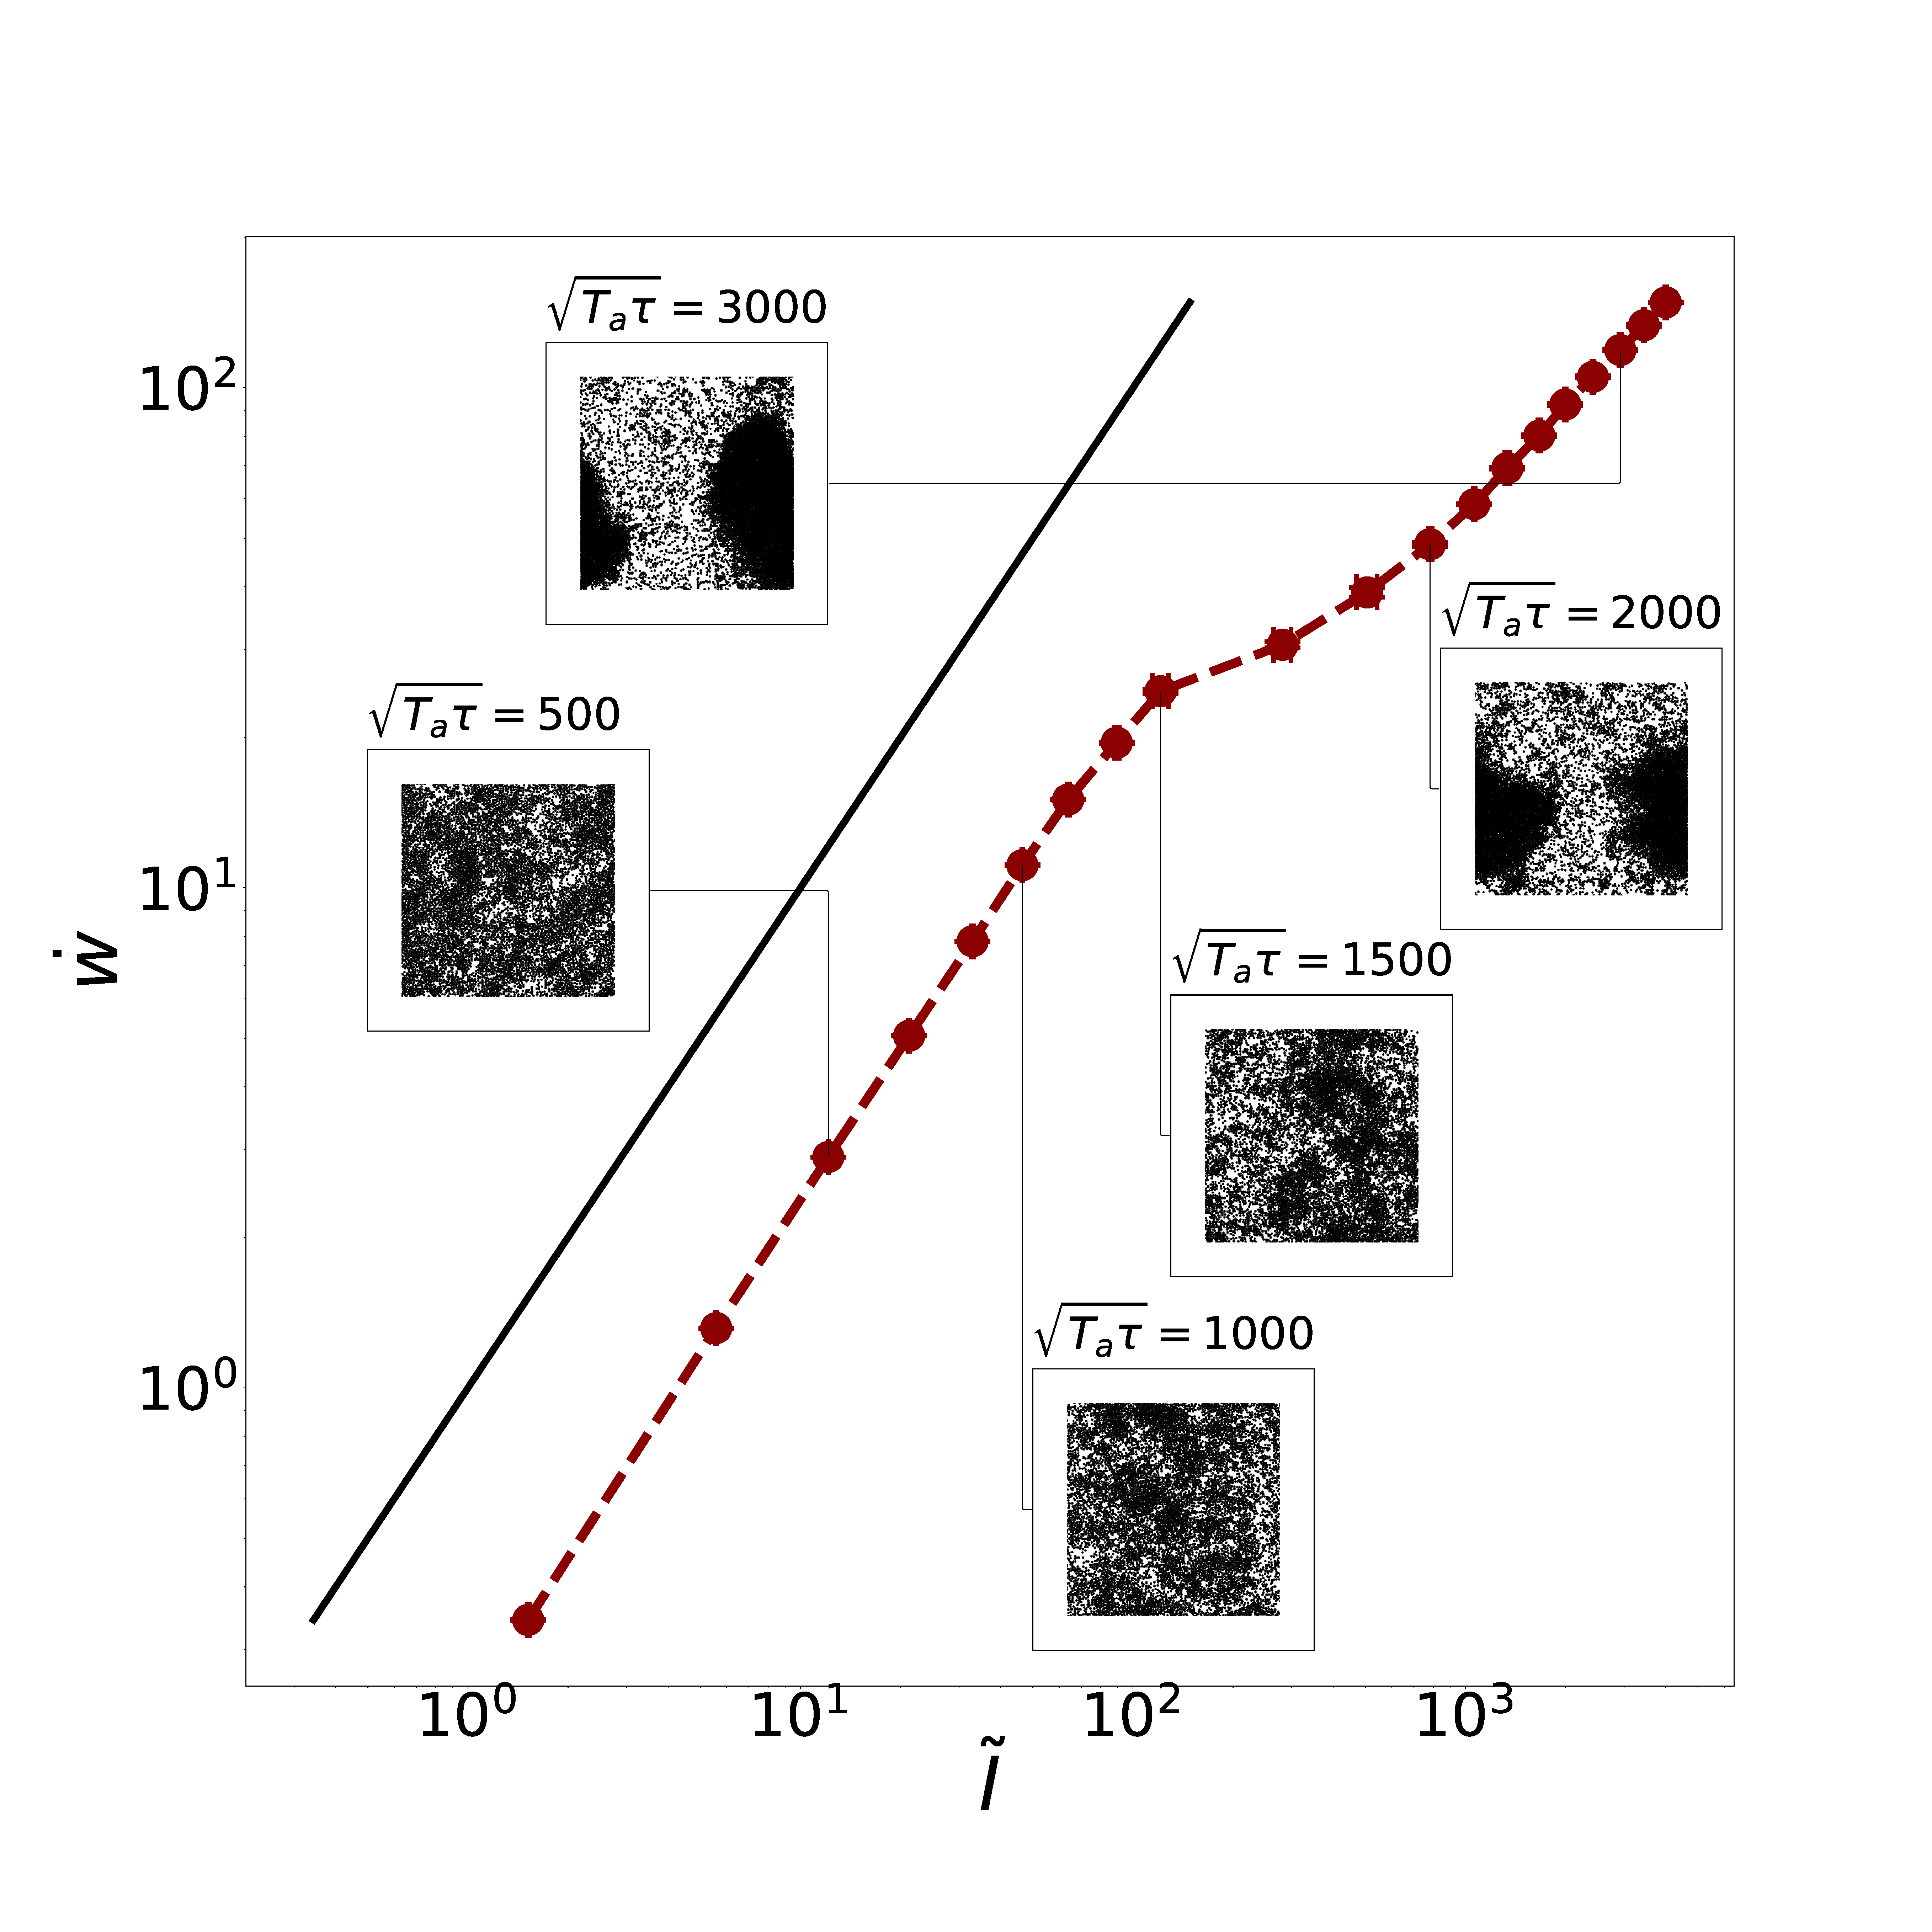
\includegraphics[scale=0.09, clip=True]{Figure_3.eps}
    \caption{The linear relationship between rate of work and $\tilde{I}$ holds up to $Pe$ values that are within 25\% of the $Pe$ where phase transition occurs (a little under 60). In the phase separated region, the linear relationship appears to still hold but with a different slope. Parameters: WCA potential, $\rho =0.75$, $\tau = 33.33$}
    \label{Fig:3}
\end{figure}
\begin{figure*}[t]
\centering
    \includegraphics[scale=0.27, clip=True]{Fig_ML_cut.pdf}
    \caption {Inferring dissipation from static configurational data. (a) The machine learning architecture consists of a convolutional layer, which performs the operation ${\bf r}_i * F(r) = \sum_{j \neq i} F(r_{ij})$, where $j$ runs over a set number of nearest neighbors. The function $F$ is expressed in a basis of Gaussian functions and the coefficients are learned by the machine. The function $F(r)$ could be expected to be learned as $\nabla u(r)^2 - \nabla^2 u(r)$, and therefore we compare the learned function with this function in the inset plots. The second layer fully connects the convolutional layer neurons, labeled as $\mathcal{I}_i$, to the output neuron through the weights $u_i$ and bias $b$:  $\sum_i u_i {\mathcal{I}_i} +b = \dot{w}$. The weights $u_i$ are constrained to be equal to ensure particle indistinguishibility. (b) The machine is trained using configurations generated at even values of $T_a$ between 0 and 12, but the value of the rate of work is predicted at both odd and even values between 0 and 12. The agreement with the real rate of work is excellent, and the $F(r)$ is also learned accurately given that we do not allow discontinuities in the learned function. Parameters: Harmonic potential, $\rho = 1$, $\tau = 1$. (c) Similar analysis as in (b). Parameters: Yukawa potential, $\rho = 0.5$, $\tau = 1$. (Insets) Representative snapshots of configurations from simulations at $T_\A=0$, $T_\A=10$ (Harmonic), and $T_\A=0$, $T_\A=30$ (Yukawa). The machine learning algorithm is able to learn the dissipation rate from such static configurational snapshots with no information related to the active ${\bf f}_i$ degrees of freedom.}
    \label{Fig:ML}
\end{figure*}
Indeed, in Fig.~\ref{Fig:2} we plot estimates of $\dot{w}$ and $\tilde I$ obtained from simulations and from our analytical theory. The simulations were performed at various values of $T_a$ ranging from $T_a=2$ to $T_a=10$, with $\tau=1.0$ and with a density of $\rho=1$. We used a short ranged interparticle potential $U({\bf r})=A (1- r)^2, r\leq 1$. The analytical estimates for $A\geq 2 K_bT$ were obtained by numerically integrating the expression for $\tilde I$ in Eq.~\ref{eq:Idef} using Eq.~\ref{eq:final_expression_gr}. In the weak interacting limit, $A=0.5 K_b T$, as we show in SI (Section C), it is possible to derive a compact closed form expression for $\tilde I$ in terms of the interaction potential. This expression was used to compute $\tilde I$ for systems with $A=0.5 K_b T$. The simulations show a linear connection between $\dot{w}$ and $\tilde I$. While the \textit{exact} values of $\dot{w}$ and $\tilde I$ predicted by the theory deviate moderately from the simulation values \textendash as might be expected from the errors in the predicted short length scale structure we noted above \textendash our theory performs surprisingly well in predicting the slope $\alpha$ for various values of $A$. 

We note that the linear connection between $\dot{w}$ and $\tilde I$ eventually fails at larger values of $T_a$ for the harmonic potential (SI Figure 2) most likely on account of the fact that the particle cores can fully overlap for sufficiently strong driving forces. However, for systems with steeper repulsive potentials, such as systems with Yukawa and WCA interparticle potentials, this linear connection works for a much larger regime (SI Figure 3). In particular, we have observed that for the WCA potential, the connection between dissipation and structure persists even in regions close to the phase transition (Fig.~\ref{Fig:3}). 

% We note that since our mean-field theory fails to accurately account for the rapid short length scale variations, and since these variations play a dominant role in systems with strongly repulsive short-ranged potentials, our theory is not able to predict exact values of $\dot{w}$ and $\tilde I$ for systems with Yukawa and WCA interparticle potentials.    -- This is an exact repeat of what we already said in the previous paragraph, starting with "While the exact values ..."} 

% However, even in these cases, the theory is still able to provide a good approximation for the longer length scale features of the non-equilibrium correlation and direct correlation function, like in Fig.~\ref{Fig:1}, for low to moderate values of the non-equilibrium activity (SI). ---  This is also repetitive and doesn't belong here


{\it Inferring dissipation from static configurations with neural networks}---The results in Fig.~\ref{Fig:2},\ref{Fig:3} show how the average dissipation rate can be inferred using just the configurational two-particle correlation function data. The purpose of this section is to construct a proof of principle neural network that can map snapshots of AOUP particles to the energy dissipation encoded in them. Such a proof of principle may form the basis for the development of a feedback control processes where the dissipation rate is tuned adaptively until the desired structure is achieved. 
To this end,  we designed a network consisting of a continuous convolutional layer followed by a dense layer (Fig. \ref{Fig:ML}a). The continuous convolutional layer is inspired by recent work on rotationally and translationally invariant networks for atomic systems \cite{tess2018}. Convolutional neural networks have been recently used in Ref \cite{Seif2020} to show how the dissipation rate is indeed connected to time reversal symmetry violations. 

We prepared 35000 snapshots using the harmonic potential and 30000 snapshots using  the Yukawa potential. These correspond to 5000 snapshots per $T_a$, where $T_a$ ranged from 0 to 12 in increments of 2 for harmonic and from 0 to 30 in increments of 6 for Yukawa. The snapshots were divided into 80\% train and 20\% validation sets, and the network was trained until we observed convergence of the validation loss (between 200 and 300 epochs of training), using the adam optimizer in keras with batch size 512. In Fig.~\ref{Fig:ML} b,c we show the agreement between the real and predicted $\dot{w}$, averaged over 10 trials. The test data reflected in Fig.~\ref{Fig:ML} b,c comes from independent simulations ran over a more fine-grained range of $T_a$'s, from which we extracted 1000 configurations per $T_a$ . The neural network is able to infer the dissipation rate with good accuracy just from configurational data. Indeed, in the prediction phase, the neural network was supplied with configurations generated at values of $T_a$ that were never used in the training phase. The neural network was able to correctly anticipate the dissipation rate $\dot{w}$ at these values of $T_a$. This calculation also independently verifies the connection between dissipation and structure noted in the previous section. We further demonstrate in Fig.~\ref{Fig:ML} b,c (inset plot) how our continuous convolution neural network is able to actually infer the form of the function that needs to be multiplied by $g(r)$ to get to the dissipation. In contrast with most existing approaches, we stress again that no information related to the polarization is required.



{\it Concluding remarks}: Our results demonstrate that the relationship between microscopic structure and dissipation rate in far-from-equilibrium AOUP systems can be predicted with better accuracy than has been previously achievable using a theory based on mean-field approximations. Crucially, this can be achieved while relying only on structural information that is time-independent and simple to measure: a neural network is able to infer the dissipation of the system very accurately by learning only from snapshots. While the close-packing interactions of strongly interacting AOUPs that arise from driving are difficult to capture fully, this work nevertheless opens the door to developing theories connecting structure and dissipation in more complex systems with a potentially large range of functions.


\acknowledgements{
This work was mainly funded by support from a DOE BES Grant DE-SC0019765 to LT and SV (theoretical and computational calculations, machine learning). \'EF acknowledges support from an ATTRACT Investigator Grant of the Luxembourg National Research Fund. We gratefully acknowledge extremely useful discussions with Pratyush Tiwary. 
}

%\begin{figure}
%    \centering
%    \includegraphics[scale=0.25, clip=True]{HarmonicA16_p1.0_Ta10_U0.40.pdf}
%    \caption{}
%    \label{Fig:n}
%\end{figure}

%\begin{figure}
%    \centering
%    \includegraphics[scale=0.25, clip=True]{Ck_A16_T10_U0.4.pdf}
%    \caption{Prediction for c(k) in a moderately driven system of harmonic disk particles %following the procedure in the text (blue), compared with predicted c(k) for the system %with no driving (red) and measured c(k) from simulation with driving (black). $\rho = %1.00, A = 16, \tau = 0.4, T_a = 10$ (blue, black); $T_a = 0$ (red).}
%    \label{Fig:n}
%\end{figure}

%\begin{figure}
%    \centering
%    \includegraphics[scale=0.25, clip=True]{HarmonicA16_p1.0_Ta30_U0.40.pdf}
%    \caption{}
%    \label{Fig:n}
%\end{figure}

%\begin{figure}
%    \centering
%    \includegraphics[scale=0.25, clip=True]{Ck_A16_T30_U0.4.pdf}
%    \caption{Prediction for c(k) in a strongly driven system of harmonic disk particles %(blue), compared with predicted c(k) for the system with no driving (red) and measured %c(k) from simulation with driving (black). $\rho = 1.00, A = 16, \tau = 0.4, T_a = 30$ %(blue, black); $T_a = 0$ (red).}
%    \label{Fig:n}
%\end{figure}

%\begin{figure}
%    \centering
%    \includegraphics[scale=0.25, clip=True]{Yukawahr_Yp0.5_Pe3_U1.00.pdf}
%    \caption{}
%    \label{Fig:n}
%\end{figure}

%\begin{figure}
%    \centering
%    \includegraphics[scale=0.25, clip=True]{YukawaCk_Yp0.5_Pe3_U1.00.pdf}
%    \caption{Prediction for c(k) in a moderately driven system of Yukawa particles (blue), %compared with predicted c(k) for the system with no driving (red) and measured c(k) from %simulation with driving (black). $\rho = 0.50, A = 50, \kappa = 4.00, \tau = 1.0, T_a = 9$ %(blue, black); $T_a = 0$ (red).}
%    \label{Fig:n}
%\end{figure}

%\begin{figure}
%    \centering
%    \includegraphics[scale=0.25, clip=True]{Yukawahr_Yp0.5_Pe6_U1.00.pdf}
%    \caption{}
%    \label{Fig:n}
%\end{figure}

%\begin{figure}
%    \centering
%    \includegraphics[scale=0.25, clip=True]{YukawaCk_Yp0.5_Pe6_U1.00.pdf}
%    \caption{Prediction for c(k) in a strongly driven system of Yukawa particles (blue), %compared with predicted c(k) for the system with no driving (red) and measured c(k) from %simulation with driving (black). $\rho = 0.50, A = 50, \kappa = 4.00, \tau = 1.0, T_a = %36$ (blue, black); $T_a = 0$ (red).}
%    \label{Fig:n}
%\end{figure}

%\begin{figure}
%    \centering
%    \includegraphics[scale=0.25, clip=True]{ShiftedYukawaCk_Yp0.5_Pe6_U1.00.pdf}
%    \caption{Prediction for c(k) in a strongly driven system of Yukawa particles (blue), %compared with predicted c(k) for the system with no driving (red) and measured c(k) from %simulation with driving (black). Compared with Fig. 8, the theoretical c(k) has along the %k axis to alignat with simulation results. $\rho = 0.50, A = 50, \kappa = 4.00, \tau = %1.0, T_a = 36$ (blue, black); $T_a = 0$ (red).}
%    \label{Fig:n}
%\end{figure}

%\begin{figure}
%    \centering
%    \includegraphics[scale=0.1, clip=True]{Plots_dW_tI_Suri_R1.00_A16.00_U1.000.pdf}
%    \caption{}
%    \label{Fig:n}
%\end{figure}



%\begin{figure}
%    \centering
%    \includegraphics[scale=0.1, clip=True]{Results_xR_yA.pdf}
%    \caption{}
%    \label{Fig:n}
%\end{figure}


\bibliography{References.bib}

\end{document}
